\documentclass[letter, 11pt]{article}
\usepackage[utf8]{inputenc}
\usepackage[english]{babel}
\usepackage{amsfonts, amsmath, amsthm, amssymb}
\usepackage[dvips]{graphicx}
\usepackage{url}
\usepackage[top=3cm,bottom=3cm,left=3.5cm,right=3.5cm,footskip=1.5cm,headheight=1.5cm,headsep=.5cm,textheight=3cm]{geometry}
\usepackage{listings}
\usepackage{color}
\usepackage{fancyvrb}
\usepackage{fancyhdr}
\usepackage{enumerate}
\usepackage{multirow}
\usepackage{hyperref}
%% to use the warpfigure capability
\usepackage{wrapfig}
%% Double spacing
\usepackage{setspace}

%%%%%%%%%%%%%%%%%%%%%%
%Estilo del documento%
%%%%%%%%%%%%%%%%%%%%%%
\pagestyle{fancyplain}

%%%%%%%%%%%%%%%%%%%%%%%%%%%%%%%%%%%%%%%%%%%
%Fancyheadings. Top y Bottom del documento%
%%%%%%%%%%%%%%%%%%%%%%%%%%%%%%%%%%%%%%%%%%%
% Recuerde que en este documento la portada del documento no posee
% numeracion, pero de igual manera llamaremos a esa primera pagina la numero
% 1, y la que viene la dos. Esto es para tener una idea de las que
% llamaremos pares e impares	
\lhead{} %Parte superior izquierda
\rhead{\bf \it UTFSM, Casa Central} %Parte superior derecha
\lfoot{JSCO} %Parte inferior izquierda.
\cfoot{} %Parte inferior central
\rfoot{\bf \it Page \thepage} %Parte inferior derecha
\renewcommand{\footrulewidth}{0.4pt} %Linea de separacion inferior
\renewcommand{\thefootnote}{\roman{footnote}}
\newtheorem*{theoremnon}{Theorem}

\begin{document}
%%%%%%%%%%%%%%%%%%%%%%%%%%%
% Tema de las referencias %
\bibliographystyle{acm}
%%%%%%%%%%%%%%%%%%%%%%%%%%

%%%%%%%%%%%%%%%%%%%%%%%%%%
%Definicion de la portada%
%%%%%%%%%%%%%%%%%%%%%%%%%%
\begin{titlepage}
    \begin{center}
	\begin{tabular}{ccc}
	    
\includegraphics[width=3cm]{img/utfsm}
	    & 
	    \hspace{-0.2cm}
	    \begin{tabular}{c}
		Universidad T\'ecnica Federico Santa Mar\'ia \\ \hline
		\vspace{0.2cm}
		Departamento de Inform\'atica\\
		\vspace{1.2cm}
	    \end{tabular}
	    \hspace{0.2cm}
	    &
            
\includegraphics[width=2cm]{img/di}
	\end{tabular}

	\vspace{1cm}
	%Titulo del Documento
	\begin{tabular}{c}
		\Huge{\sc{Testing, Detection and Possible}}\\\\
		\Huge{\sc{Solutions for the Bufferbloat}}\\\\
		\Huge{\sc{Phenomenon on Networks.}}\\\\
		\Large{\sc{State of Art}}\\\\
	\end{tabular}

    	\vspace{2cm}
	\Large{\sc{JUAN S. CATALAN OLMOS}}\\
	\vspace{2cm}
	\large{Definici\'on de Tema de Memoria}\\
	\large{para optar al T\'itulo de:}\\
	\large{INGENIERO CIVIL INFORMATICO}\\
	\vspace{2cm}
         	\normalsize{Profesor Gu\'ia: Horst H. von Brand Skopnik}\\
         	\normalsize{Profesor Coreferente: Ra\'ul Monge Anwandter}\\
	%Fecha
    
    \vspace{2cm}
    \normalsize{\sc{\today}}\\
    \normalsize{\sc{Valpara\'iso, Chile}}\\
    \end{center}
\end{titlepage}


\newpage

\tableofcontents
\newpage
\listoffigures
%\listoftables

\newpage

\doublespacing
%section Intro
\section{Introduction}

According to the reports published by SUBTEL to the first half of 2013,
\textit{12.8} per 100 inhabitants have access to broadband
Internet\cite{OCDE}.  This steady growth is largely due to the emergence of
new applications such as streaming video and music, online gaming and
bandwidth intensive applications.

Not long ago, the links had a much more limited bandwidth than they have
today. With the evolution of electronics and telecommunications,
speeds have increased dramatically. With the current level of data flowing
through the network, it is important to control congestion that
might occur. This is one of the tasks of the routers.

It is important to remember that the traffic in a network is inherently
bursty, the role of the buffers in the router is to smooth the flow of
traffic. Without any buffering, to allocate the bandwidth evenly would be
impossible. But there are some problems with current algorithms; they use
tail-drop based queue management that has two big drawbacks: 1.- lockout 2.-
full queue that impact with a high queue delay.

Current low hardware prices make memory cheap,
and with the ``more is better'' mentality have led to the inflation and
proliferation of buffers everywhere\cite{NicholsJacobsonCQD}. When a router
joins two networks with different bandwidths, each packet is squeezed down in
bandwidth, it must stretch out in time since its size stays constant. When
the queue starts to grow, more and more memory is deployed leading to
massive standing queues. It turns out that this is a recipe for Bufferbloat.
Evidence of Bufferbloat has been accumulating over the past decade, but its
existence has not yet become a widespread cause for concern.

Bufferbloat creates large delays but no improvement in throughput. It is not a
phenomenon treated by queueing or traffic theory, which unfortunately results
in it being almost universally misclassified as congestion. The \textit{\gls{Bufferbloat}}
problem, making the window match the pipe size, is hard to address. Window
sizes are chosen by senders while queues manifest at bottleneck gateways.


As mentioned by Jim Gettys and Kathleen Nichols;
\textit{Today's networks are suffering from unnecessary latency and poor
system performance. The culprit is Bufferbloat, the existence of excessively
large and frequently full buffers inside the network. Large buffers have been
inserted all over the Internet without sufficient thought or testing. They
damage or defeat the fundamental congestion-avoidance algorithms of the
Internet's most common transport protocol. Long delays from Bufferbloat are
frequently attributed incorrectly to network congestion, and this
misinterpretation of the problem leads to the wrong solutions being
proposed}\cite{GettysNichols}.

The objective of this thesis work is checking the effects of
Bufferbloat phenomenon, test the impact that it has on different networks
and to propose solutions. To accomplish this, it first requires to
address the following general objectives:

\begin{itemize}
	\item To define the \textit{Bufferbloat} phenomenon, and explain the impact that it could have on latency and \gls{Throughput}(related to \gls{System Throughput}) in Internet.
	\item To detect its presence by measurements of the latency and throughput in a TCP/IP Network.
	\item To propose solutions in the implementation of a network where the existence of excessively large and frequently buffers are detected
\end{itemize}

In order to archive theses objectives:

\begin{itemize}
\item Develop appropriate tests to be able to prove the existence of \textit{Bufferbloat}
\item To test and differentiate the possible causes of the excessive latency and throughput reduction in a TCP/IP LAN and check how much is generated by \textit{Bufferbloat} or by a miss-configuration
\item To propose configuration of the TCP parameters in a Linux based machine or an algorithm that can help to minimize the phenomenon.
\end{itemize}

Chapter 2 explains the basis on which TCP was developed and
the fundamentals for the current operation of the Internet. The conservation
principle upon which all communication protocols are based will be explained.
It also describes each of the four phases of TCP.

In Chapter 3 we will review one of the most important components for the
communication and the main place where the packages are stored: the Routers.
We will analyze how their queues have a destructive size for
communication, why they are stalled at full capacity and cause excessive
latency. We also consider how to define the appropriate buffer size in a router.

Chapter 4 presented a technique developed to deal more efficiently with
actively congestion that could generate not only on endpoints but also on
routers. This technique is Active queue management (AQM). How the first
algorithms, such as RED and BLUE, were implemented and mention
CODEL which aims to solve the Bufferbloat phenomenon; This failures points,
in both TCP and AQM, are synthesized and analyze. All this will be presented in
Chapter 5.

Chapter 6 aims to define the methodology and tools that will be used to
perform each of the tests to determine the existence and the effects of
Bufferbloat. Each test is defined by its propose starting with some general
tests to check the behavior and sanity of the network and moving to a more
user-related effects of the Bufferbloat. All the tools used are Open Source
projects available for all commercial operative systems. In Chapter 7 the
results of all tests are presented, leading to the conclusions of this work in
chapter 8.


%end intro
%section Foundation
\section{The Bufferbloat Foundations}
\subsection{The TCP Protocol \cite{rfc793}\cite{rfc2001}}
%http://www.linktionary.com/c/congestion.html
%http://condor.depaul.edu/jkristof/technotes/congestion.pdf 

The Transport Control Protocol or TCP is main transport protocol of the
internet, providing reliable host to host communication over unreliable
transport media\cite{rfc793}. The advantages of its connectionless design,
flexibility and robustness provides reliable, ordered delivery of a stream of
bytes from a program on one computer to another program on another computer,
but for that, the cost are: the needed of careful design so it provides a good
service under heavy loads. Many modifications has been done since it was
originally defined in 1981.

The root idea of any algorithm related to transport connections must be based
into the ``\textit{packet conservation principle}". This principle claims:

\begin{defn}
A new packet isn't put into the network until an old packet leaves.
\end{defn}


\subsubsection{Slow-Strart Algorithm\cite{rfc879}\cite{rfc2460}}
\indent Old TCPs implementation, would start a connection with the sender injecting multiple segments into the network, up to the window size advertised by the receiver.  This action has no implications if the two host are into the same LAN. While this is OK when the two hosts are on the same LAN; but in the Internet, this schema isn't valid. As is know, between the two end points are routers and getaways, and the flow of packages is not constant, between the two end points some links could be slower than others, and some intermediate buffer's queues could run out of space.\\

The algorithm to starts this ``\textit{clock}'' and to avoid this congestion
 \begin{wrapfigure}{r}{0.5\textwidth}
  \begin{center}
    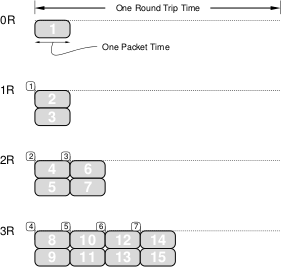
\includegraphics[width=0.48\textwidth]{img/slowstart}
  \end{center}
  \caption{The Chronology of a Slow-Start.\cite{Jacobson:1988:CAC:52325.52356}}
  \label{slowstart}
\end{wrapfigure}
is called \textit{slow start}. It is the responsible to gradually increase the amount of data that is in transit by observing that the a new package is injected into the network until the acknowledgment of a previous packages as arrives from the other end. In other words, it is used to avoid sending more data than the network is capable of transmit.\\

Slow start adds a variable window to the sender's TCP:  the congestion window, called ``\textit{cwnd}'' to the per-connection state.  When a new connection is established or restarting after a loss connection with a host, the congestion window is initialized to one segment, with the size of two times the maximum segment size (MMS)\footnote{The study of MMS is out of the scope of this paper, but more info could be found in \cite{rfc879} and \cite{rfc2460}} .  Each time an ACK is received, the congestion window is increased by one segment (1 MMS).  The sender can transmit up to the minimum of the congestion window and the advertised window.  The congestion window is flow control imposed by the sender, while the advertised window is flow control imposed by the receiver.  The former is based on the sender's assessment of perceived network congestion; the latter is related to the amount of available buffer space at the receiver for this connection.\\

The sender starts by transmitting one segment and waiting for its ACK. When that ACK is received, the congestion window is incremented from one to two, and two segments can be sent.  When each of those two segments is acknowledged, the congestion window is increased to four as seen in figure \ref{slowstart}. Here, the gray numbered boxes are packages and the white are the corresponding ACK. As each ACK arrives, two packages are generated, one for the ACK package that left the ``\textit{pipe}'' and one because an ACK opens the congestion window by one. This provides an exponential growth, it takes time \textbf{$Rlog_2 W$}\cite{Jacobson:1988:CAC:52325.52356}, where R is the round trip time and W is the window size. Although it is not exactly exponential because the receiver may delay its ACKs,typically sending one ACK for every two segments that it receives.\\

At some point the capacity of the internet can be reached, and an intermediate router will start discarding packets.  This tells the sender that its congestion window has gotten too large. Early implementations performed slow start only if the other end was on a different network.  Current implementations always perform slow start.\\


\subsubsection{The Congestion Avoidance Algorithm \cite{rfc2309}\cite{rfc2581}}
\indent In the ``\textit{slow start}" phase, if a when a lost occurs, half of the current window is saved as a Gresham a variable that is
 used to determine whether the slow start or congestion avoidance algorithm is used to control data transmission. After this, the \textit{cwnd} is set again to 1 and start to grown until it reaches the ssthresh again. Now, TCP goes into congestion avoidance mode, where for each ACK increases the cwnd in 1/cwnd. A congestion can occur when data arrives at a router whose output capacity is less than the sum of the inputs.  Congestion avoidance is a way to deal with lost packets.\\
	
This algorithm makes a fundamental assumption: \textit{the packet loss caused by damage is very small (much less than 1\%), therefore the loss of a packet signals congestion somewhere in the network between the source and destination}.  Two are the indication of package lost: a timeout occurring and the receipt of duplicate ACKs.\\

A good congestion avoidance strategy, must have two components: 1.- The endpoints should know when a congestion is about to occur or occurring into the network, and 2.- If a signal that alert the congestion is received, the network's utilization must decrease and increases if the signal isn't received.\\

When a networks is getting congested, the queue lengths will start to increase exponentially (because of slow-start). The system will collapse if the network doesn't throttle back the traffic sources at leas as quick as the queues are growing. The way that the network announces via dropped packets when demand is excessive, but says nothing if a connection is using less than its fair share. This is also another problem because causes underbuffering, also causing that the resources are not fully under full use.\\

The implementation of congestion avoidance is as simple as slow start, but with a slight difference\cite{Jacobson:1988:CAC:52325.52356}. The steps are:
\begin{enumerate}
\item On any timeout, set \textit{cwnd} to half the current window size. This produces a multiplicative decrease.
\item On each ack for new data, increase \textit{cwnd} by 1/\textit{cwnd}. Now cwnd has an additive increment so now the growth becomes linear.
\item When sending, send the minimum of the receiver's advertised window and \textit{cwnd}.
\end{enumerate}

A window of size cwnd packets will generate at most cwnd ACKs in one round trip time. Thus an increment of 1/cwnd per ACK will increase the window by at most one packet in one RTT. In TCP, windows and packet are in bytes so the increment translates to segsize*segsize/cwnd, where segsize is the segment size and cwnd is maintained in bytes.\\

Congestion avoidance and slow start are independent algorithms with different objectives.  But when congestion occurs TCP must slow down  its transmission rate of packets into the network, and then invoke slow start to get things going again. In practice they are implemented together. So, if cwnd is less than or equal to ssthresh, TCP is in slow start; otherwise TCP is performing congestion avoidance. Slow start continues until TCP is halfway to where it was when congestion occurred (since it recorded half of the window size that caused the problem ), and then congestion avoidance takes over.\\


\subsubsection{The Router's Congestion Avodance Complements}
After the ``congestion collapse" and with the growth in the last few decades of
 \begin{wrapfigure}{l}{0.5\textwidth}
  \begin{center}
    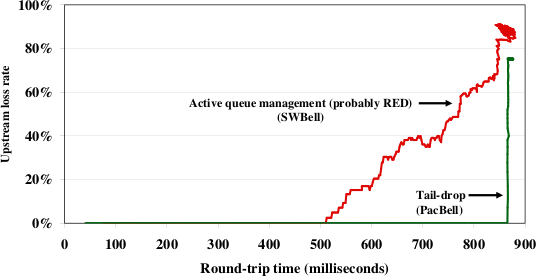
\includegraphics[width=0.48\textwidth]{img/overflows}
  \end{center}
  \caption{How Tail-drop management and RED AQM overflows\cite{Dischinger2007CRB}}
  \label{tdredof}
\end{wrapfigure}

Internet, it has become clear that the TCP congestion avoidance mechanisms,
while necessary and powerful, are not enough to provide a fully safe service,
and the control that can be accomplished from the edges of the networks has
proof that has a limit. So, in order to obtain a good service in all
circumstances, some mechanisms in the routers to complement this endpoint
congestion avoidance mechanisms are needed.\\

Two classes of router algorithms related with congestion avoidance control can
be distinguished: ``queue management" and ``scheduling" algorithms. While the
first one manage the length of packet queues by dropping packets when necessary
or appropriate, the second one determine which packet to send next, and are used
to manage the allocation of bandwidth among flows. It is important to notice
that while this two mechanisms are closely related, the performance that they
address are rather different and should be seen as complementary, and not as
replacements for each other.\\



\begin{enumerate}
\item \textbf{Managing the Routers Queue:} As we have seen in previous section, the traditional way to manage router queue
is, after set a maximum length for the queue, accept packages until this length
is reached, and then drop subsequent packages until a packet from the stack as
been transmitted. This technique is called ``tail drop", and has served the
Internet well enough for years, but it has two important drawbacks:\\

\begin{itemize}
\item It allows, in some situations, a single or few flows to monopolize the
queue space, preventing other connections from getting room in the queue.
\item The signaling is produced only when the queue is full, so it allows queue
to maintain almost full status for long periods.
\end{itemize}

If queue is full or almost full, an arriving burst will cause multiple packets to
be dropped, an this behavior can produce a global synchronization of flows
throttling back followed by sustained period of lowered link utilization, which
will impact in a reduce of overall throughput, and if a long flows arrives in
that period, the lock-out of the queue.\\

Besides tail drop, another two techniques can be applied in these situations.
The ``random drop on full" will produce that the router drops a randomly selected
packet from the full queue, which requires an $O(N)$ walk through the queue, when a
new packet arrives. Under the ``drop front on full", the router drops the packet
at the front of the queue. Either of these solve the lock-out problem, but
neither solves the full-queue.\\

\item \textbf{Active Queue Management and Random Early Detection} In the current Internet, dropped packets are used as a critical mechanism to
notify a end node when a congestion is presented. So, if a router is capable to
drop packets before the queue is full, and the end nodes take actions before the
buffers overflow, the full-queue problem is solved. This proactive approach is
know as ``active queue management" (AQM) and allows routers to control when and how
many packets to drop before buffers overflow.\\

For responsive flows, AQM can provide:
\begin{itemize}
\item reduce number of packets dropped in routers
\item provide lower-delay interactive service
\item avoid lock-out behavior
\end{itemize}

One AQM algorithm for routers is called ``Random Early Detection" or RED. The
algorithm drops arriving packets probabilistically, which increases as the
estimated average queue size grows, so it approach is based on the ``recent
past" events.\\

The RED algorithm consists of two main parts:

\begin{itemize}
\item Estimation of the average queue size
\item Packet drop decision
\end{itemize}

RED's particular algorithm for dropping is the culprit in the performance
improvement. 

\end{enumerate}

\subsection{Latency}
% 2.- Latency: When a new package arrives, it has to wait to the full queue get processed before its time, this way the package spent extra time waiting in the queue.
The latency a packet experiences in a network is made up of transmission
delay (the time it takes to send it across communications links), processing
delay (the time each network element spends handling the packet) and queuing
delay (the time spent waiting to be processed or retransmitted). But large
buffers only increase latency, and this only causes conflict with the needs
of nowadays applications.

Once packets in-fly reach a bottleneck, they begin to pool. Because the
characteristics already explained, more and more packets are coming, and this
queue continues to increase, which leads that each new arriving packet spending
more time in the queue than the predecessor packet, which means an
increase in the latency. Eventually, packets start to be dropped,
notifying the hosts of the presence of congestion on the path.

As stated in \cite{Dischinger2007CRB}, it is quite common to find these high-
latency queues in the last mile. The causes can be many, but among the most
common are both link quality at homes, as different implementations of traffic
shaping methods implemented by ISPs, or massive buffers set by the latter to
avoid loss of data, which can add a delay of up to several milliseconds.
Bottlenecks at the Internet's edge can easily move between the wireless
access (when its bandwidth is slow) and the provider's up-link, both of which
can have highly variable bandwidths.

For networks that use coaxial cable, multiple clients concatenated their
upward flows in a single transmission, resulting in a burst with a large
volume of data, which can led to a high fluctuation in latency. This
concatenation can also generate jitter time, which can be produce a miss
interpretation for some protocols of incipient congestion and cause to enter
into congestion control avoidance too early. The other type of highly used
networks are the DSL, which the more distance is between the supplier reduces
its transmission rate. That is why it is needed advanced signal processing and
error correction algorithms which can lead to high packet propagation delays.


\newpage

%end section Fundation
%section Characterization
\section{Characterization of Bufferbloat}

\subsection{Backbone Routers}

As we already know, all internet routers contains buffers to hold packets during times of congestion. A widely used rule-of-thumb states that each link need a buffer of size $B = \overline{RTT} x C $, where $\overline{RTT}$ is the average round trip time of a flow passing across the link, and C is the data rate of the link. The main characteristic of bufferbloat is the existence of excessively large and frequently full buffers inside the network. Large buffers have been inserted all over the Internet without sufficient thought or testing, so router buffers are the single biggest contributor to uncertainty in the Internet.\\

The rule-of-thumb come from a desire to keep the link as busy as possible so, the throughput of the network is always as big as possible. But, because the way that TCP works, no matter how big the buffer is at the bottleneck link, TCP will cause the buffer to overflow.\\ 

Overbuffering is a bad idea for two reasons:
\begin{enumerate}
\item It complicates the design of high-speed routers, leading to higher power consumption, more board space, and lower density.
\item It increases end-to-end delay in the presence of congestion
\end{enumerate}

As seen in 2.2, large buffers only increases latency, and this only causes conflict with the needs of real time applications.\\

The most important fact of sizing a buffer is to make that sure that while the sender pauses, the router buffer doesn't go empty and force the bottleneck to go idle. Again, the idea is to keep as much throughput as possible so the use of the link is fully utilized. The buffer will avoid to idle if the first packet from the sender shows up at the buffer just as it hits empty. In previous section, we define that after a lost is detected, the cwnd is set to half of is last value, so if we denote as $(W_{max} /2)/C$ the amount of time that packets are sent in congestion phase, and as $B/C$ the time that takes a buffer with size B to drain, the size of a buffer B needed is $B \leq (W_{max} /2)$.\\

Also from \cite{main:ref:1}, we can see that the rule-of-thumb doesn't longer apply to backbone routers, and a better estimator of the size of a buffer with n flows would be no more than $B = (\overline{RTT}xC)/\sqrt{n}$. With the assumption that short-flows plays a very small effect, and that the buffer size is dictated by the number of long flows, this factor will be proof that routers are much longer than they need to be, possible by two order of magnitude.


\subsection{Residential BroadBand Networks}
It is well know that residential networks are often the bottleneck in the last
mile access to the Internet Infrastructure. This could be because the ISP's of
both of the most popular ways to access (DSL and cable networks) to internet
today, use traffic shaping methods and ,as seen in previous sections, deploy
massive queues that can delay packets for several hundred milliseconds.\\

Both shares the asymmetric bandwidths; they downstream bandwidth is higher than
their upstream bandwidth, but in cable networks a single coaxial cable shares
multiple customers, they can concatenate multiple upstream packets into a single
transmission, which result in short bursts at high data rates, so the latency
can heavily fluctuate. This concatenation can produce a jitter time, that under
high network load can be higher than end-to-end jitter over the entire path
under normal load, which can be produce a miss interpretation for some protocols
of incipient congestion and cause to enter into congestion control avoidance too
early.\\

In the other hand, in DSL networks, the maximum data transmission
rate falls with increasing distance from the head, thus in order to boost the
transmission rate, DSL relies on advanced signal processing and error correction
algorithms which can lead to high packet propagation delays .\\




\newpage

%end section Characterization
%section Test
\section{Experimental Work}
The goal of the experiments outlined in this section is to examine different
residential and public networks with the objective to proof the existence of the
phenomenon under an uncontrolled scenario. This will be done by running a set of
tests with different tools, first to define and characterize the network, then
to measure and compare how the network behave with and without load. More
specifically, the factor to be tested is the latency under load and analyzed to
identify if the latency that occurs is due to an excess of buffers or due to
some other problem.

This section aims to explain the setup that will be used to perform the tests,
the selected tools for each of these tests and what is to be achieved and 
expected from each one of these tests.


\subsection{The Test Setup}
The tests were ran under a pseudo controlled environment, using one
physical  machine and a second virtual machine hosted on the first machine. These
systems runs under a regular OS without any modifications. Also, for some tests two other devices will be
added,  one acting as an Iperf Server and a regular Android Tablet that will
be used to add some extra load to the network when the Ethernet cable is used
as medium.

All of these tests will be carried out in a real-world scenario, where no
packet  prioritization is done by the server against our flows, the routes can
vary between each iteration of the same test, and many different flows will
collide with other flows from different sizes and types. Nor there is more
information about how the flows are treated by the queue manager algorithms or
about how they are  configured.

\subsubsection{Hardware Characterization}

\begin{description}

\item [Physical Machine]: \hfill \\
The physical machine runs as host OS, Windows 7 SP1, that works with an Intel(R)
Core(TM) i7-2670QM CPU \@ 2.20GHz with 8GB of available RAM. This machine will 
always be connected through its wireless adapter, a \textit{Broadcom Corp. 
BCM4313 802.11b/g/n Wireless LAN Controller (rev 01)}. The Ethernet controller 
is a \textit{Realtek Semiconductor Co., Ltd. RTL8111/8168 PCI Express Gigabit 
Ethernet controller (rev 06)} adapter, and will be bridged to the virtual 
machine for some tests.

\item[Virtual Machine]: \hfill \\
The virtual machine is hosted using VMWare Player 6.0.1, with 4 processors 
assigned for use plus 4GB of RAM, and with the Ethernet adapter connected only
for certain tests. The OS selected is a Debian based OS called Kali Linux, and
using the kernel release identified as Debian 3.12.6-2kali.

The wireless adapter is a AIR-802 USB adapter with Zydas chipset and a TP-link
8dbi antenna. This adapter is directly connected to the virtual machine and
hooked to the physical machine without the USB extension, this way any extra
signal  loss is avoided. 

\item[Iperf Server]: \hfill \\ 
This is a VPS hosted by Digital Ocean
\footnote{\url{https://digitalocean.com}} with 512MB Ram, 20GB SSD Disk, and
located in New York data center. This machine runs Ubuntu 12.04.3 x64 under
KVM software using as a processor an Intel Hex-Core 3 GHz.

\end{description}

The idea of using an external device to connect the virtual machine to the 
network and not using a bridged configuration provided by software, is mainly 
because with an USB device the machine will take care of all the management and 
administration of the device, avoiding any possibility that the host machine 
modifies or manages any flow. Also, by using a second machine to overload the 
uplink avoids overflow the queue on the machine that is performing 
the tests. With this, it is expected to minimize the possibility that our 
testing machine is causing extra latency, either by the saturation of the 
wireless channel, or by the queue in the traffic control subsystem into the 
kernel. 

For the tests, the Bufferbloat community\cite{bloat} has created a set of best 
practices\cite{tg12} to follow so the results are consistent and repeatable, 
but in this case, computers and routers will not be modified as it will attempt 
to analyze what an every-day-user experience. Those practices will be taken in 
consideration if it is the QOS present in routers and deactivate as recommended.
 


\subsection{Tools Definition}
The tools used for the benchmark were selected by the capability to
determine  the presence of the Bufferbloat phenomenon in the network of
study. So, with this as a main consideration, the
tools selected for  the benchmark will be chosen by the complexity and
accuracy to measure and  determine the RTT into an IP/TCP connection, and how
hard is to consistently  replicate the results under similar contexts. Other
tools were selected to help  determine, characterize, and prove the capability
of the network to cause  Bufferbloat.

\newpage 

The tools selected to be used in this tests are the following:

\begin{itemize}
    \item Speedtest test by Ookla
    \item Netalyzr by ICSI
    \item Iperf Tool with Tcptrace/Xplot.org
    \item Page Benchmarker extension for Google Chrome
    \item Smokeping Latency Tool
\end{itemize}

\subsubsection{Speedtest}

Developed by Ookla\footnote{\url{https://www.ookla.com/about}}, this tool is used
for most of the ISPs and many users in Chile to test their broadband's
connections globally. It can be used not only in their website 
\href{http://www.speedtest.net}{\emph{www.speedtest.net}} but also on Android,
iOS or Windows Phone. A command line interface developed in Python can be used 
too for testing Internet bandwidth.

The server selected to perform every test, either has or not the
fastest ping, is the one hosted by the Pontificia Universidad Cat\'olica de
Valpara\'iso (this host is the default selected most of times by the site also).  

\subsubsection{Netalyzer}

For end-users, little is revealed about how ISPs manage their networks. That is
why since 2009 ICSI has developed Netalyzr, a ``two click '' tool developed to
test networks that runs in web browser as a Java applet. Once downloaded, the
applet contacts the back-end server using a range of protocols and mechanisms
employed as part of the testing, and then conducts a series of tests. Once
completed, it uploads its findings to the back-end where they are distilled
into a detailed report breaking down the findings into correctly operating
aspects, those that show potential signs of trouble, and those that are
downright broken. Figure \ref{netalyzr_ex} is an example of the output.

\begin{wrapfigure}{r}{0.5\textwidth}
	\begin{center}
		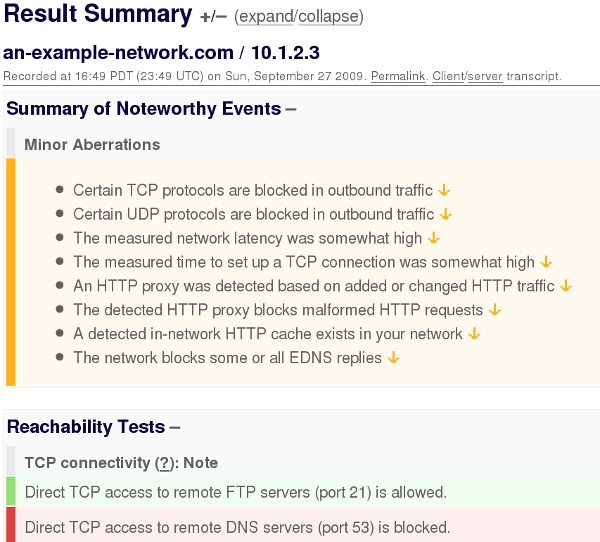
\includegraphics[width=0.48\textwidth]{img/netalyzr_ex}
	\end{center}
	\caption[Result Summary example from Netalyzr]{Result Summary example from Netalyzr. Source:
	\url{www.dslreports.com}}   
	\label{netalyzr_ex} 
\end{wrapfigure}

The primary goal in developing Netalyzr's tests was to provide a new kind of
diagnostic tool, \emph{one that particularly illuminates under what sort of
restrictions a user's Internet connection operates, like both forms of filtering
(blocking) and proxying imposed by the user's ISP, and performance issues that
arise from the nature of the user's Internet access setup}\cite{netalyzr}. Among
the performance considerations, Netalyzr's measures are packet loss, latency,
bandwidth. Also, it compute in-path forwarding device buffer size by comparing
small-packet latencies under idle and loaded states in networks (the perfect
time to occur Bufferbloat). Other tests like general TCP and UDP service
reachability are performed.

\subsubsection{Iperf}
Iperf is a well known and commonly used network testing tool. It can create a
TCP and UDP data streams and measure the bandwidth and the quality of a network
link. It can perform multiple tests like Latency, Jitter or Datagram Loss.

Iperf basically tries to send as much information down a connection as quickly
as possible reporting on the throughput achieved. This tool is especially useful
in determining the volume of data that links between two machines can supply.
This two machines define the network, one acting like a server and the second as
the client. For this scenario, the server will be the VPS that only will receive
the Iperf connections (also will be running ssh but without further
interaction). The VM Linux machine will work as an Iperf Client.

As mentioned in Iperf users mailing list ``\emph{When one runs TCP tests,
there are 2 things that block Iperf from having clear view of real throughput:
buffering on sender's side (TCP/IP stack) and TCP behavior itself (acking).
What Iperf can measure is the pace with which it sends data to TCP/IP stack;
TCP/IP stack will only accept data from application when buffers are not full.
If the buffer is huge, Iperf will see high throughput initially, then it will
drop. If there's congestion or retrasmission going on, Iperf will see it as
lower throughput}''\cite{iperfmaillist}, but the data generated by Iperf won't
be further analyzed because the  idea behind using this tool is a TCP's packet
generator. This means that the packets generated by  Iperf will captured and
analyzed with tcpdump, tcptrace and xplot.org.

\subsubsection{Page Benchmarker}
Page Benchmarker is a Google Chrome extension that intent to test page load 
time performance within Chrome. Measures time-to-first-paint, overall page load 
time, KB read/written, and several other metrics, and with its capability to 
clear the cache and existing connections between each page load, makes this 
tool one of the main sources of income to analysis.

\subsubsection{Smokeping}
SmokePing is a latency logging and graphing tool that consists of a running 
daemon which organizes the latency measurements and a CGI which presents the 
graphs. SmokePing give us the ability to measure latency and packet loss 
in the current network, and with RRDtool, is capable to maintain a long term 
data store and to draw different graphs with the giving up-to-the-minute 
information on the state of each network connection.

Smokeping can be configured to perform a wide range of latency measurement 
probes each one directed to an independent target or over a set of targets 
selected for each proof.


\subsection{Test Description}
description


%end section Test
\section{Results}

\section{Conclusions}
By analyzing all of the work done for this thesis, it is possible to conclude
that the objective of it was achieved considering the same frame of reference
as the criteria defined at the beginning of it being the \emph{objective of
checking the effects of Bufferbloat phenomenon, test the impact that it has in
on different networks and to propose solutions}. To accomplish
this, it first required to address the following general objectives:

\begin{itemize}
	\item To explain the \emph{Bufferbloat} phenomenon, and explain the impact that it could have over latency and throughput in Internet.
	\item To detect the presence by empirical measure of the latency and throughput in a TCP/IP Network.
	\item To propose possible solutions in the implementation of a network where the existence of excessively large and frequently buffers are detected.
\end{itemize}

Thanks to the various tests it was possible to demonstrate the presence and
feel the effects of \emph{Bufferbloat} in some networks. While the common
factor in them at first sight is their low bandwidth, you can not directly
assign this as a cause, as also contrary cases that had a bad performance
determined by physical effects such as routers were in poor condition or
environmental interference.

As proven in this thesis and corroborated in \cite{MathisMacroCAA}, in
general, a low latency network is wanted in order to exchange  messages between a server and a client. Since low latency make us feel
a faster web surfing and enables better performance in online games and VoIP
technology.

It is clear that the farther away a clients is from the server, the latency
will be higher, but what if we put more and more load to the network, how much
the latency can go up to? Having 12 times the latency when the network
overload is not normal and as mentioned by \emph{Jim Gettys} several times,
the culprit is Bufferbloat.

The effects on latency and navigation are catastrophic growing to full
charging time in minutes or even generate timeout sites.  If we take
today's world where it is more and more common to see applications that make use of
high bandwidth, makes it almost impossible navigating multiple users with these
characteristics. Then, two users on the same network using such applications
should take turns to ensure a smooth operation.

Also from \cite{main:ref:1} and \cite{Vu-Brugier}, we can see that the rule-of-thumb of sizing routers $B = (\overline{RTT}xC)$ doesn't longer apply. With
routes which have sizes much larger buffers than required, all it does is slow
down and hinder the passage of trading floors. The larger the buffer size, the
longer it takes for a packet to go through it, not adding any value in the
packet transfer and only adding additional latency.

In the past days networks had much lower performance than they are today,
so as \emph{Bufferbloat} alike phenomena were more difficult to detect
because their effects were not as visible. Today with the advance of
technology and the use of tools that feed us with information almost
instantaneously, any change or modification at any point within the
communication channel is evident, and why not say is magnified even to make
some systems collapse.

The complexity of deploying new algorithms into production environments is
such that no matter how many tests are performed over new algorithms, the
conditions under development environments will hardly match. Also doing testing
in production environments is too hard and too complex\cite{Vu-Brugier},
and if tests are not well designed can affect users in a hard way.

Thanks to Codel, and Bufferbloat community is possible to propose an effective
solution to the phenomenon of Bufferbloat. Although while this phenomenon has been studied for a couple of years, the solutions are not yet fully proven,
but these solutions are designed
for modern systems (e.g.. Codel requires BQL recommended for Linux kernel 3.5
onwards), so there will always be some systems vulnerable to its effects. Apply
QoS and bandwidth limiting for some applications are the
most common and easy to implement recommendations for any user, regardless of
the operating system on which they are working.

It is also important to keep a regular check of all the components in our
networks, not only to our computer. Effects of routers in evil, or using
technologies like wireless with the boom of recent years in homes fact that
interference between emitters is much more common than years ago, can be
determining factors in achieving this long-awaited win the last game shooter,
or close the business of our lives through a video conference.

Much is still to be done in this field. As example, the analysis in specific of
how the three different flows (Elephant, mice and
ant)\cite{HaElephants, evolvshortlongflows} are affected by big buffers
and prioritize smaller flows can help fix some of the issues like DNS
resolution, but how they react when the whole network is under the effects of
\emph{Bufferbloat}? The effects change if this occurs at a last-mile-router
or at a back-bone?

Thanks to studies as done by Hoiland-Jorgensen\cite{TokeLinux}, is that a
better understanding of how the Linux Kernel reacts to \emph{Bufferbloat}, but
this follows up to all Linux based OS? With the advance of technology, new
devices are getting cheaper and most people can have access to them. Well
known is the case of Open-Wrt\cite{openwrt}, that is a Linux distribution for
embedded devices. Projects like Cero-WRT\cite{cerowrt}, can help to the
community to fight against \emph{Bufferbloat} in every piece that is
involved on the communication. But will this help in all devices? As example,
Arduino Yun is a microcontroller board, with an Atheros processor that
supports a Linux distribution based on OpenWrt named OpenWrt-Yun. The board
has built-in Ethernet and WiFi support. So, will this board behave well under
high consumption of bandwidth too? Also the effects of \emph{Bufferbloat}
under Windows machine are not well known. Beside the recommendations of the
Bufferbloat community\cite{windowstips} not much information can be found
about it. Study the effects under laying the use of
CTCP\cite{Tan06compoundtcp}\cite{4146841} will be a good starting point.



\section{Further Work}
further


%%%%%%%%%%%%%%%%%%%%%%%%%%%
%incluyo referencias
\bibliography{references,rfc}{}
%%%%%%%%%%%%%%%%%%%%%%%%%%%%

\end{document}
